\subsection{Supplementary Services}

As the other branches of the prototyping where happening, the need for additional services and infrastructure arose to 
support the development of the prototype as well as to increase the general usability of the prototype. 
This section will especially describe the services which help to make this prototype a more complete solution.


\begin{figure}[htb]
    \centering
    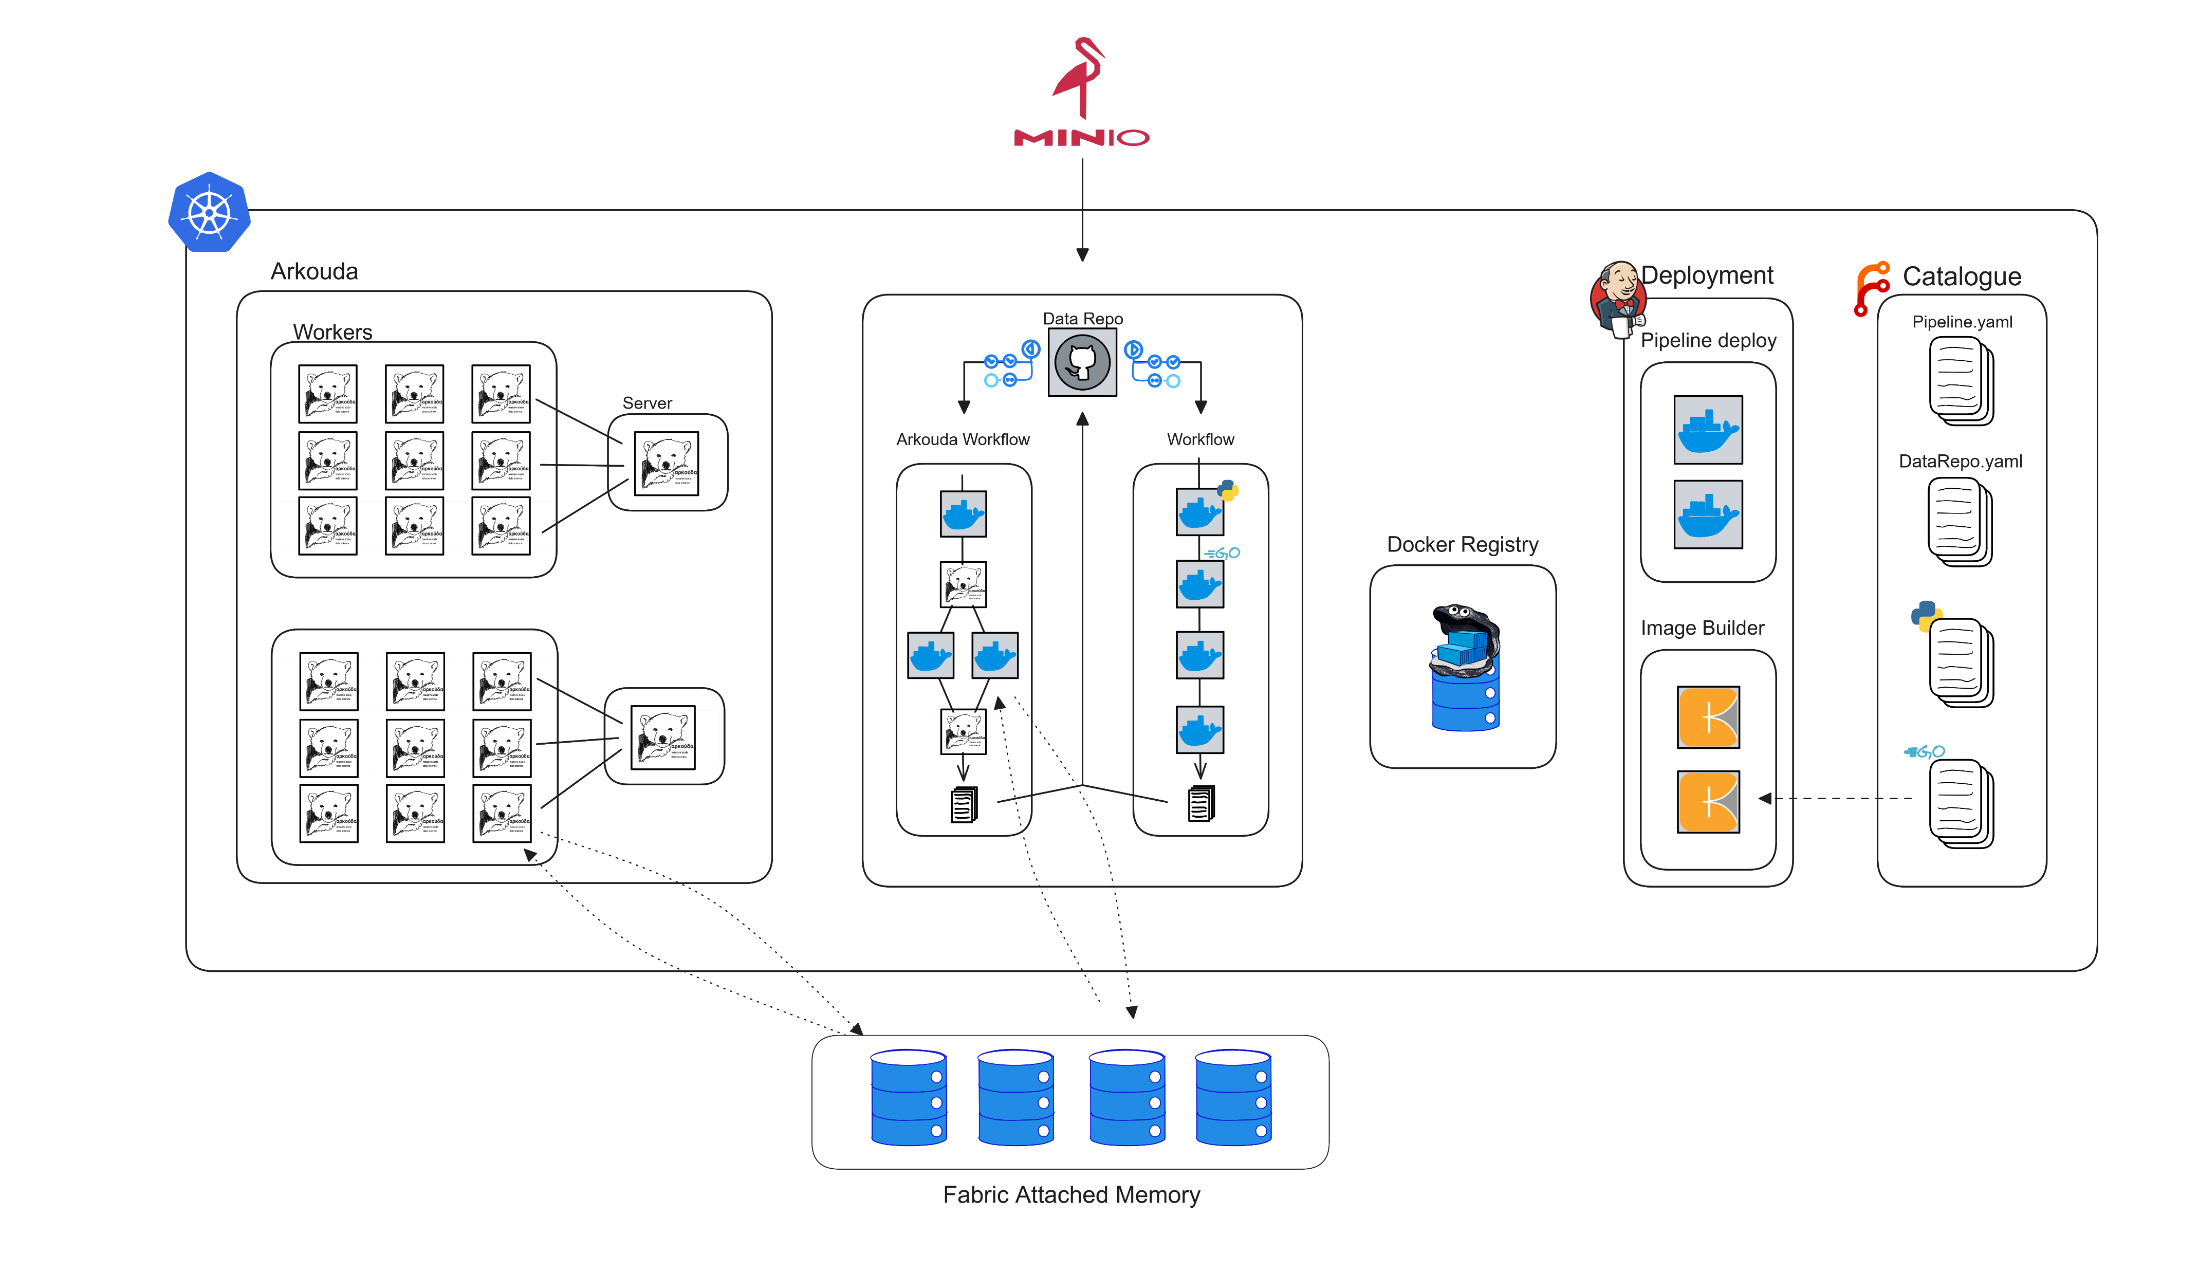
\includegraphics[width=17cm]{graphics/pachykouda_complete.png}
    \caption[Pachyderm High-Level Architecture]{Pachyderm High-Level Architecture}
    \label{abb:pachyderm_complete}
\end{figure}

\subsubsection{Docker Registry}

One thing that was quite apparent from the get go, was the need for a central docker registry.
As Pachyderm does not manage the docker images itself, but relies on the user to provide them somehow externally.

During the first iterations when the development was being done on Minikube as described in \ref{minikube}, the internal Registry 
of the node was enough.
But as soon as we moved over to the Heydar system keeping the Hosts internal registries in sync was of course not feasible,
Therefore we added a private docker registry to the cluster \footcite{kumarHowSetupPrivate2020}.
The deployment config is based on the official docker registry helm chart\footcite{Dockerregistry10Phntom} and can be found at \ref{appendix:docker_registry_config}.

\subsubsection{Frogejo Catalogue}

One if the main goals of this project was to create a tool that is accessible to the end user,
and therefore the need for a catalog of available workflows arose.
The idea was to create something similar to the Clasp catalogue\footcite{sayersCLoudApplicationServices2015} but for the Pachyderm ecosystem.
Meaning that users can share, search and deploy workflows from a central catalog, without having to worry about the underlying infrastructure.

Having \ac{HPC} software in a completely contained and version system directly addresses many of the original problem statements,
described in \ref{ProblemStatement}, especially the problem of reproducibility, environment management and the lack of portability.
A first 

\subsubsection{Jenkins CI/CD Pipeline}
